\documentclass[12pt, letterpaper]{article}
\usepackage[utf8]{inputenc}
\usepackage{graphicx}
\usepackage{hyperref}

\title{Rapport personnel pour le cours de compréhension de programme}
\author{Chaolei CAI}

\begin{document}


\begin{titlepage}
    \maketitle
\end{titlepage}

\tableofcontents
\section{Introduction}
Ce document est le rapport personnel de CAI Chaolei pour le cours compréhension de programme\\
Je suis dans le groupe 1 avec Ramu Danabal, Omar Hammouche, Predrag Kostiec. \\
Notre projet portait sur l'outil Gimp, plus précisement la version 2.10.14\\
L'environnement de test et d'utilisation est la distribution Linux : Manjaro-XFCE 64bit 18.1.3\\
Un dépôt GitHub a été crée pour ce projet, il peut être consulté depuis ce lien \url{https://github.com/pkostic-git/gimp-2-10-12-p8}


\section{Objectives}
1/Modification de la boîte à outils, plus précisement de l'outil "Text", il faut le modifier afin qu'il affiche "groupe 1 text" au lieu de "Text."\\
2/Modifier la police et la taille de la police de defaut.\\
3/Ajouter un nouveau 'outil' ou 'boutton' qui change la taille de la police utilisée par une autre taille.\\
4/Ajouter un nouveau 'outil' ou 'boutton' qui ouvriras une fênetre de dialog qui afficheras le résultat de la commande "ls -l" depuis le répertoire courant.

\section{Démarrage du projet}
Au début, le groupe a choisit de mettre l'accent sur la recherche car la machine virtuelle de test n'était pas encore mise en place, j'ai commencé à régler ma machine virtuelle sur la distribution Ubuntu 18.04LTS.\\
Je me suis porté volontaire pour mettre en place la machine virtuelle car c'était un peu compliqué pour les autres de l'installer. Ils se sont donc misent à faire des recherches sur les objectives sur internet.
 Maleuheusement, il n'y a pas vraiment de sujet ou de tutoriel sur internet qui nous apprends à customiser gimp. Il y'a certe le wiki de Gimp mais cela ne fut pas d'une grande aide.\\


\section{Compilation}
Il y avait un problème de version très pénible avec Ubuntu quand j'essayais de compiler les codes sources, en effet cela est due au gestionnaire de paquet d'Ubuntu qui ne dispose pas des dernières versions de librairie demandé par Gimp.\\
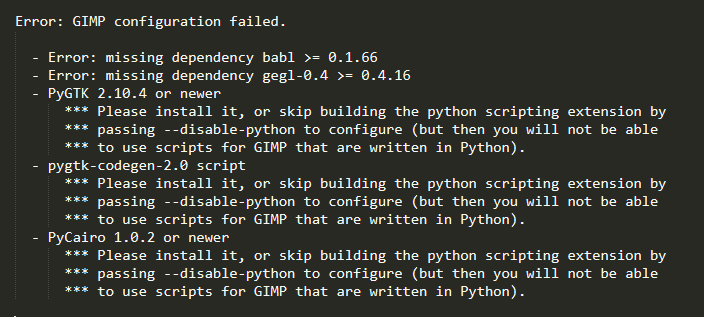
\includegraphics[width=\linewidth]{c1.png}
J'ai crée dans le dépot un fichier DEPENDENCIES.txt dans le répertoire gimp-2.10.12/ , il contient tous les noms de paquet que j'ai pu installé sur la machine.\\
Le problème était que Gimp requière les bibliothèque babl et gegl, mais apt ne disposait que des versions anciennes.
J'ai due donc télecharger le code source pour babl et gegl afin de les installer manuellement, et là je suis tombé dans le piège des dépendances de paquet, l'un d'entre eux demandait svg, ninja et meso. Comme d'habitude apt ne satisfait pas les exigences de versions nécessaire, encore un fois il fallait compiler le code source manuellement... De nouvelles dépendences etc.\\
Finallement, le problème fut réglé en changeant de distribution, je suis donc passé à la distribution Manjaro, ce dernier utilisait pacman comme gestionnaire de paquet. J'ai beaucoup plus d'habitude avec pacman que apt comme j'utilise Arch Linux pour travailler. Plus besoin de se casser la tête pour les versions car pacman propose toujours la version la plus récente sauf indication de l'utilisateur.
C'est ainsi que avec rien à installé de plus, Gimp compilait et je l'ai enfin installé.

\section{Proposition hypothèse}
Nous nous somme basé sur ce que nous avons fait dans l'exercice précedent, en repassant à la vue les répertoires, nous avons décidé de se concentrer sur le répertoire app/tools et app/code car app contenait le code source de Gimp, tools a probablement un lien proche avec la boîte à outils et core contenait des fonctions primaires de Gimp.\\


\end{document}
